%! ~~~ Packages Setup ~~~ 
\documentclass[]{article}


% Math packages
\usepackage[usenames]{color}
\usepackage{forest}
\usepackage{ifxetex,ifluatex,amsmath,amssymb,mathrsfs,amsthm,witharrows,mathtools}
\WithArrowsOptions{displaystyle}
\renewcommand{\qedsymbol}{$\blacksquare$} % end proofs with \blacksquare. Overwrites the defualts. 
\usepackage{cancel,bm}
\usepackage[thinc]{esdiff}
\usepackage{tabularx}


% tikz
\usepackage{tikz}
\newcommand\sqw{1}
\newcommand\squ[4][1]{\fill[#4] (#2*\sqw,#3*\sqw) rectangle +(#1*\sqw,#1*\sqw);}


% code 
\usepackage{listings}
\usepackage{xcolor}

\definecolor{codegreen}{rgb}{0,0.35,0}
\definecolor{codegray}{rgb}{0.5,0.5,0.5}
\definecolor{codenumber}{rgb}{0.1,0.3,0.5}
\definecolor{codeblue}{rgb}{0,0,0.5}
\definecolor{codered}{rgb}{0.5,0.03,0.02}
\definecolor{codegray}{rgb}{0.96,0.96,0.96}

\lstdefinestyle{pythonstylesheet}{
	language=Python,
	emphstyle=\color{deepred},
	backgroundcolor=\color{codegray},
	keywordstyle=\color{deepblue}\bfseries\itshape,
	numberstyle=\scriptsize\color{codenumber},
	basicstyle=\ttfamily\footnotesize,
	commentstyle=\color{codegreen}\itshape,
	breakatwhitespace=false, 
	breaklines=true, 
	captionpos=b, 
	keepspaces=true, 
	numbers=left, 
	numbersep=5pt, 
	showspaces=false,                
	showstringspaces=false,
	showtabs=false, 
	tabsize=4, 
	morekeywords={as,assert,nonlocal,with,yield,self,True,False,None,AssertionError,ValueError,in,else},              % Add keywords here
	keywordstyle=\color{codeblue},
	emph={object,type,isinstance,copy,deepcopy,zip,enumerate,reversed,list,set,len,dict,tuple,print,range,xrange,append,execfile,real,imag,reduce,str,repr,__init__,__add__,__mul__,__div__,__sub__,__call__,__getitem__,__setitem__,__eq__,__ne__,__nonzero__,__rmul__,__radd__,__repr__,__str__,__get__,__truediv__,__pow__,__name__,__future__,__all__,},          % Custom highlighting
	emphstyle=\color{codered},
	stringstyle=\color{codegreen},
	showstringspaces=false,
	abovecaptionskip=0pt,belowcaptionskip =0pt,
	framextopmargin=-\topsep, 
}
\newcommand\pythonstyle{\lstset{pythonstylesheet}}
\newcommand\pyl[1]     {{\lstinline!#1!}}
\lstset{style=pythonstylesheet}

\usepackage[style=1,skipbelow=\topskip,skipabove=\topskip,framemethod=TikZ]{mdframed}
\definecolor{bggray}{rgb}{0.85, 0.85, 0.85}
\mdfsetup{leftmargin=0pt,rightmargin=0pt,innerleftmargin=15pt,backgroundcolor=codegray,middlelinewidth=0.5pt,skipabove=5pt,skipbelow=0pt,middlelinecolor=black,roundcorner=5}
\BeforeBeginEnvironment{lstlisting}{\begin{mdframed}\vspace{-0.4em}}
	\AfterEndEnvironment{lstlisting}{\vspace{-0.8em}\end{mdframed}}


% Deisgn
\usepackage[labelfont=bf]{caption}
\usepackage[margin=0.6in]{geometry}
\usepackage{multicol}
\usepackage[skip=4pt, indent=0pt]{parskip}
\usepackage[normalem]{ulem}
\forestset{default}
\renewcommand\labelitemi{$\bullet$}
\usepackage{titlesec}
\titleformat{\section}[block]
{\fontsize{15}{15}}
{\sen \dotfill (\thesection)\dotfill \she}
{0em}
{\MakeUppercase}
\usepackage{graphicx}
\graphicspath{ {./} }


% Hebrew initialzing
\usepackage[bidi=basic]{babel}
\PassOptionsToPackage{no-math}{fontspec}
\babelprovide[main, import, Alph=letters]{hebrew}
\babelprovide[import]{english}
\babelfont[hebrew]{rm}{David CLM}
\babelfont[hebrew]{sf}{David CLM}
\babelfont[english]{tt}{Monaspace Xenon}
\usepackage[shortlabels]{enumitem}
\newlist{hebenum}{enumerate}{1}

% Language Shortcuts
\newcommand\en[1] {\begin{otherlanguage}{english}#1\end{otherlanguage}}
\newcommand\sen   {\begin{otherlanguage}{english}}
	\newcommand\she   {\end{otherlanguage}}
\newcommand\del   {$ \!\! $}
\newcommand\ttt[1]{\en{\footnotesize\texttt{#1}\normalsize}}

\newcommand\npage {\vfil {\hfil \textbf{\textit{המשך בעמוד הבא}}} \hfil \vfil \pagebreak}
\newcommand\ndoc  {\dotfill \\ \vfil {\begin{center} {\textbf{\textit{שחר פרץ, 2024}} \\ \scriptsize \textit{נוצר באמצעות תוכנה חופשית בלבד}} \end{center}} \vfil	}

\newcommand{\rn}[1]{
	\textup{\uppercase\expandafter{\romannumeral#1}}
}

\makeatletter
\newcommand{\skipitems}[1]{
	\addtocounter{\@enumctr}{#1}
}
\makeatother

%! ~~~ Math shortcuts ~~~

% Letters shortcuts
\newcommand\N     {\mathbb{N}}
\newcommand\Z     {\mathbb{Z}}
\newcommand\R     {\mathbb{R}}
\newcommand\Q     {\mathbb{Q}}
\newcommand\C     {\mathbb{C}}

\newcommand\ml    {\ell}
\newcommand\mj    {\jmath}
\newcommand\mi    {\imath}

\newcommand\powerset {\mathcal{P}}
\newcommand\ps    {\mathcal{P}}
\newcommand\pc    {\mathcal{P}}
\newcommand\ac    {\mathcal{A}}
\newcommand\bc    {\mathcal{B}}
\newcommand\cc    {\mathcal{C}}
\newcommand\dc    {\mathcal{D}}
\newcommand\ec    {\mathcal{E}}
\newcommand\fc    {\mathcal{F}}
\newcommand\nc    {\mathcal{N}}
\newcommand\sca   {\mathcal{S}} % \sc is already definded
\newcommand\rca   {\mathcal{R}} % \rc is already definded

\newcommand\Si    {\Sigma}

% Logic & sets shorcuts
\newcommand\siff  {\longleftrightarrow}
\newcommand\ssiff {\leftrightarrow}
\newcommand\so    {\longrightarrow}
\newcommand\sso   {\rightarrow}

\newcommand\epsi  {\epsilon}
\newcommand\vepsi {\varepsilon}
\newcommand\vphi  {\varphi}
\newcommand\Neven {\N_{\mathrm{even}}}
\newcommand\Nodd  {\N_{\mathrm{odd }}}
\newcommand\Zeven {\Z_{\mathrm{even}}}
\newcommand\Zodd  {\Z_{\mathrm{odd }}}
\newcommand\Np    {\N_+}

% Text Shortcuts
\newcommand\open  {\big(}
\newcommand\qopen {\quad\big(}
\newcommand\close {\big)}
\newcommand\also  {\text{, }}
\newcommand\defi  {\text{ definition}}
\newcommand\defis {\text{ definitions}}
\newcommand\given {\text{given }}
\newcommand\case  {\text{if }}
\newcommand\syx   {\text{ syntax}}
\newcommand\rle   {\text{ rule}}
\newcommand\other {\text{else}}
\newcommand\set   {\ell et \text{ }}
\newcommand\ans   {\mathit{Ans.}}

% Set theory shortcuts
\newcommand\ra    {\rangle}
\newcommand\la    {\langle}

\newcommand\oto   {\leftarrow}

\newcommand\QED   {\quad\quad\mathscr{Q.E.D.}\;\;\blacksquare}
\newcommand\QEF   {\quad\quad\mathscr{Q.E.F.}}
\newcommand\eQED  {\mathscr{Q.E.D.}\;\;\blacksquare}
\newcommand\eQEF  {\mathscr{Q.E.F.}}
\newcommand\jQED  {\mathscr{Q.E.D.}}

\newcommand\dom   {\mathrm{dom}}
\newcommand\Img   {\mathrm{Im}}
\newcommand\range {\mathrm{range}}

\newcommand\trio  {\triangle}

\newcommand\rc    {\right\rceil}
\newcommand\lc    {\left\lceil}
\newcommand\rf    {\right\rfloor}
\newcommand\lf    {\left\lfloor}

\newcommand\lex   {<_{lex}}

\newcommand\az    {\aleph_0}
\newcommand\uaz   {^{\aleph_0}}
\newcommand\al    {\aleph}
\newcommand\ual   {^\aleph}
\newcommand\taz   {2^{\aleph_0}}
\newcommand\utaz  { ^{\left (2^{\aleph_0} \right )}}
\newcommand\tal   {2^{\aleph}}
\newcommand\utal  { ^{\left (2^{\aleph} \right )}}
\newcommand\ttaz  {2^{\left (2^{\aleph_0}\right )}}

\newcommand\n     {$n$־יה\ }

% Math A&B shortcuts
\newcommand\logn  {\log n}
\newcommand\logx  {\log x}
\newcommand\lnx   {\ln x}
\newcommand\cosx  {\cos x}
\newcommand\cost  {\cos \theta}
\newcommand\sinx  {\sin x}
\newcommand\sint  {\sin \theta}
\newcommand\tanx  {\tan x}
\newcommand\tant  {\tan \theta}
\newcommand\sex   {\sec x}
\newcommand\sect  {\sec^2}
\newcommand\cotx  {\cot x}
\newcommand\cscx  {\csc x}
\newcommand\sinhx {\sinh x}
\newcommand\coshx {\cosh x}
\newcommand\tanhx {\tanh x}

\newcommand\seq   {\overset{!}{=}}
\newcommand\slh   {\overset{LH}{=}}
\newcommand\sle   {\overset{!}{\le}}
\newcommand\sge   {\overset{!}{\ge}}
\newcommand\sll   {\overset{!}{<}}
\newcommand\sgg   {\overset{!}{>}}

\newcommand\h     {\hat}
\newcommand\ve    {\vec}
\newcommand\lv    {\overrightarrow}
\newcommand\ol    {\overline}

\newcommand\mlcm  {\mathrm{lcm}}

\DeclareMathOperator{\sech}   {sech}
\DeclareMathOperator{\csch}   {csch}
\DeclareMathOperator{\arcsec} {arcsec}
\DeclareMathOperator{\arccot} {arcCot}
\DeclareMathOperator{\arccsc} {arcCsc}
\DeclareMathOperator{\arccosh}{arccosh}
\DeclareMathOperator{\arcsinh}{arcsinh}
\DeclareMathOperator{\arctanh}{arctanh}
\DeclareMathOperator{\arcsech}{arcsech}
\DeclareMathOperator{\arccsch}{arccsch}
\DeclareMathOperator{\arccoth}{arccoth}
\DeclareMathOperator{\atant}  {atan2} 

\newcommand\dx    {\,\mathrm{d}x}
\newcommand\dt    {\,\mathrm{d}t}
\newcommand\dtt   {\,\mathrm{d}\theta}
\newcommand\du    {\,\mathrm{d}u}
\newcommand\dv    {\,\mathrm{d}v}
\newcommand\df    {\mathrm{d}f}
\newcommand\dfdx  {\diff{f}{x}}
\newcommand\dit   {\limhz \frac{f(x + h) - f(x)}{h}}

\newcommand\nt[1] {\frac{#1}{#1}}

\newcommand\limz  {\lim_{x \to 0}}
\newcommand\limxz {\lim_{x \to x_0}}
\newcommand\limi  {\lim_{x \to \infty}}
\newcommand\limh  {\lim_{x \to 0}}
\newcommand\limni {\lim_{x \to - \infty}}
\newcommand\limpmi{\lim_{x \to \pm \infty}}

\newcommand\ta    {\theta}
\newcommand\ap    {\alpha}

\renewcommand\inf {\infty}
\newcommand  \ninf{-\inf}

% Combinatorics shortcuts
\newcommand\sumnk     {\sum_{k = 0}^{n}}
\newcommand\sumni     {\sum_{i = 0}^{n}}
\newcommand\sumnko    {\sum_{k = 1}^{n}}
\newcommand\sumnio    {\sum_{i = 1}^{n}}
\newcommand\sumai     {\sum_{i = 1}^{n} A_i}
\newcommand\nsum[2]   {\reflectbox{\displaystyle\sum_{\reflectbox{\scriptsize$#1$}}^{\reflectbox{\scriptsize$#2$}}}}

\newcommand\bink      {\binom{n}{k}}
\newcommand\setn      {\{a_i\}^{2n}_{i = 1}}
\newcommand\setc[1]   {\{a_i\}^{#1}_{i = 1}}

\newcommand\cupain    {\bigcup_{i = 1}^{n} A_i}
\newcommand\cupai[1]  {\bigcup_{i = 1}^{#1} A_i}
\newcommand\cupiiai   {\bigcup_{i \in I} A_i}
\newcommand\capain    {\bigcap_{i = 1}^{n} A_i}
\newcommand\capai[1]  {\bigcap_{i = 1}^{#1} A_i}
\newcommand\capiiai   {\bigcap_{i \in I} A_i}

\newcommand\xot       {x_{1, 2}}
\newcommand\ano       {a_{n - 1}}
\newcommand\ant       {a_{n - 2}}

% Other shortcuts
\newcommand\tl    {\tilde}
\newcommand\op    {^{-1}}

\newcommand\sof[1]    {\left | #1 \right |}
\newcommand\cl [1]    {\left ( #1 \right )}
\newcommand\csb[1]    {\left [ #1 \right ]}

\newcommand\bs    {\blacksquare}

%! ~~~ Document ~~~

\author{שחר פרץ}
\title{היסטוריה $\sim$ מרכיבי הלאומיות $\sim$ כרטיסי "שנה טובה"}
\begin{document}
	\maketitle
	\section{}
	הסיפור הכללי שאיגרות אלו מספרות, הוא סיפור של מימוש חזון התנועה לאומיות של היהודים – הציונות. בפרט, הן מראות את הקשיים בהקמת הארץ, הצבאיים, החלקאיים, וגם מראים את הפן הדתי וההיסטורי של התנועה הלאומית. בגלויות בהן מוצגים אנשים, נראה את האידיאל של הפועל והעובד הציוני בארץ. כולן מהללות את המדינה ואת התנועה הלאומית, על מאפייניה השונים. 
	\section{}
	\begin{center}
		\begin{tabularx}{\textwidth}{|X|X|X|l|}
			\hline \textbf{מנורה, תורה ושופר} באיגרת הראשונה, הם סמלים מובהקים של הדת היהודית. & \textbf{תפילה בכותל}, באיגרת השנייה – מסורת יהודית עם הקשר היסטורי דתי. & \textbf{התכנסות לארוחת שישי} סביב שולחן עם כלים ואוכל יהודי מסרותי, כמו חלה, פמוטים, יין ומברך עם \textbf{כיפה} (באיגרת החמישית) & \hfil \textbf{דת} \hfil \\
			\hline \textbf{הכותל} הוא סמל היסטורי של העם היהודי, שמייצג חוזק שנשאר לאורך זמן. & 
			\multicolumn{2}{>{\hsize=\dimexpr2\hsize+2\tabcolsep+\arrayrulewidth\relax}X|}{באיגרת השלישית, מצויים שדות חלקאיים תחתם הכיתוב "תל אביב התרצ"ג/ב", כלומר גם בעת פרסום הגלויה היה זה היסטוריה. בגלויה מוצג אדם עובד על אדמת חול, והיא מסמלת את \textbf{העבודה הקשה שהובילה לבניית העיר}, והארץ בכלל. }  & \hfil \textbf{היסטוריה} \hfil\\
			\hline בברכה השנייה, יש \textbf{עובד אדמה} שמפזר זרעים ומפריח את השממה. & באיגרת הרביעית, אישה נושאת את דגל ישראל על רקע \textbf{שדות פתוחים וירוקים} המייצגים את הארץ. & \textbf{הכותל} הוא מאפיין מובהק של הארץ, ונמצא בירושליים – שטח אדמה שיהודים כמהו להגיע אליו במשך שנים. & \hfil \textbf{קשר לאדמה} \hfil\\
			\hline \multicolumn{2}{>{\hsize=\dimexpr2\hsize+2\tabcolsep+\arrayrulewidth\relax}X|}{במרבית האגרות, נמצא כיתוב גם בעברית וגם באגנלית. נסיק, שככל הנראה הופנו לקהל יעד שאינו דובר עברית בלבד, והוספת \textbf{הכיתוב בשפה העברית} נוספו כדי להדגיש את השפה המשותפת של העם היהודי.  } & \textbf{ספר התורה} באגרת הראשונה, במשך שנים היה מקור העברית היחיד של יהודים רבים. על כריכתו מצויים אותיות הא"ב, עוד סמל של השפה העברית. 
			& \hfil \textbf{שפה} \hfil\\
			\hline באגרת השישית והאחרונה, מוצג \textbf{צה"ל} בגאון וכיתוב ענק מאחורה של 'צה"ל', עם \textbf{סמל הצבא}, \textbf{כלים צבאיים} ו\textbf{רמתכ"לים לשעבר} (משה ודיין, וממה שהשוותי בויקיפדיה, חיים בר־לב). 
			& \textbf{חייל} באגרת החמישית, עליו סמלי הצבא כמו \textbf{כומתה} ו\textbf{מדים}, בארוחת שישי ביחד עם משפחתו – כמו ומנסים להגיד שבמשפחה ה"ציונית האידיאלית" המוצגת באגרת ישנו בהכרח חייל. & & \hfil \textbf{צבא ובטחון} \hfil\\
			\hline \multicolumn{3}{>{\hsize=\dimexpr3\hsize+3\tabcolsep+\arrayrulewidth\relax}X|}{ כמצוין לעיל, באגרת האחרונה ה\textbf{הרמתכ"לים לשעבר} שלאחר מכן נהפכו להיות \textbf{חברי כנסת}, הם חלק בלתי־נפרד מהשלטון באותה התקופה. } & \hfil \textbf{שלטון} \hfil\\
			\hline \multicolumn{2}{>{\hsize=\dimexpr2\hsize+2\tabcolsep+\arrayrulewidth\relax}X|}{באגרת הרביעית, מאחורי האישה עומדים \textbf{מפעלי חשמל} עם טורבינות מעשנות, עמודי חשמל ומפעלים בבניה. באותה התקופה, היכולת לייצר חשמל בארץ נחשבה לחדשנות, ממנה התושבים רצו לראות עוד בעתיד. גם \textbf{בניינים בבנייה} מצויים באגרת. } & באגרת האחרונה, צה"ל מוצג בגאווה. יחד עם המטוסים החדישים, הנצחון במלחמות בתקופה וגאוות החיילים, ננביע שהמטרה היא לספק עתיד טוב יותר למדינה הצעירה. & 
			\hfil \textbf{תקווה לעתיד טוב} \hfil \\
			\hline 
		\end{tabularx}
	\end{center}
	\section{}
	\begin{center}
		\begin{tabularx}{\textwidth}{|X|X|l|}
			\hline \hfil \textbf{המאפיין} \hfil & \hfil \textbf{תיאור המאפיין} \hfil & \hfil \textbf{כיצד מתבטא בגלויות}  \\
			\hline 
			הלאום היהודי גאה במסורות ארוכות השנים שלו, בחגים, בסמלים הדתיים, ובאובייקטים שמייצגים אותה. השורשים הללו מקורם בטקסטי החכמים, בתורה, ובמסורות שהתגבשו לאורך השנים. &
			בברכות חוגגים את ראש השנה (מסורת), והם שופעות בסמלים לאותן המסורות המפורטים תחת "דת" למעלה, ובנוסף דגש על ירושליים (אנשים בכותל) וגאווה בתורה (ספר תורה, אנשים מתפללים ועוד). הם הסמלים וההיסטוריה של התנועה הלאומית. & 
			
		 \hfil \textbf{גאווה במסורת ובהיסטוריה} \hfil \\
		 \hline 
			לעם היהודי הייתה זיכה לארץ ולירושליים זמן רב, והתחזקה עם עליית הציונות ושכנוע האנשים שהחלום יכול להפוך למציאות. היא הטריטוריה של התנועה הלאומית. & באגרות מפוזרות תמונות של הארץ, עיתים ירוקה באופן מוגזם, ועיתים דווקא מודגש החול והגולמיות שבא. גם תמונות בירושליים בנמצא. ניכר כי יש חשיבות רבה לאדמה הזו, שמוצגת בגאווה. פירוט רב יותר נמצא תחת "קשר לאדמה" בסעיף הקודם. &  \hfil \textbf{אהבת הארץ} \hfil \\
			\hline 
			בציונות נכחה התרבות החלוצית. כלומר, היא עודדה הקמת ישובים חדשים, הגנה על ישובים קיימים, עבודת אדמה וקיום עצמי. זאת, לנגד דמות ה"יהודי הישן", הסוחר שנודד בין ערים. & בבולים מודגש הצבא, עבודת האדמה והקמת תל־אביב – כולם הם חלק בלתי נפרד מהאופי החלוצי של הישוב היהודי בתחילתו, התרבות באותה התקופה. &  \hfil \textbf{התרבות החלוצית} \hfil \\
			\hline 
			השפה הייתה מאפיין שאיחד את העם היהודי במשך תקופה ארוכה. גם בזמנים שזו לא הייתה השפה המדוברת, ביום־יום, יהודים עד ידעו קרוא וכתוב בעברית על מנת ללמוד את התנ"ך – בכך, בעברית היוותה מעין "עוגן" לתרבויות שונות רבות שהתערבבו לכדי הזהות הציונית. & הברכות, ואף אלו שכנראה מופנות לקהל יעד שאינו דובר עברית (כי כוללת כיתוב באנגלית) מקפידות לכלול גם ברכה בעברית. התנ"ך (שקשרו לשפה מתואר בתיאור) מופיע גם בחלק מהגלויות. &  \hfil \textbf{שפה – עברית}  \hfil \\
			\hline 
			חדשנות גם היא חלק מהתרבות הציונית. העם היהודי שבארץ ישראל שאף עוד מההתחלה להישגים גבוהים – ייצור חשמל בארץ, פיתוח טכנולוגיות צבאיות, בניית מפעלים ועוד & באחת מהברכות ניתן לראות מאחורי אישה, נפרסים לאורך השגות עמודי חשמל ומפעלים, כסמן לטכנולוגיה שהצלחנו לממש. &  \hfil \textbf{חדשנות} \hfil \\
			\hline
		\end{tabularx}
	\end{center}
	
	\section{}
	אם הייתי צריך לעצב ברכה, ובציוחד לאור המלחמה, הייתי מדגיש את ההישגים של החיילים ואת החשיבות בשובם הביתה. בפרט, הייתי מדגיש את האלמנט של גאווה בצבא ובבטחון, וגם מעטר באלמנטים יהודיים מסורתיים כדי לשוות לאגרת מראה של ברגת שנה טובה. הייתי משלב גם אלמנט של דו־קיום, בנסיון להראות שאפשר לחיות בשלום עם שכיננו, על־אף המלחמה. 
	
	\section{}
	עצבתי את האגרת הבאה באמצעות AI. השתמשתי במודל Dall$\cdot$E 3 של חברת openAI. לאחר מספר בקשות קיבלתי פלט שאני יחסית מרוצה ממנו, והשתמשתי בכלי AI נוספים כדי להסיר כל מיני אלמנטים בפלט שפחות אהבתי (כמו טקסט לא קריא, או דברים נוספים שלא בקישתי מה־AI להוסיף).
	
	בתמונה רואים איש צבא מחבק ילדה, כמו והוא שב הבייתה לאחר המלחמה הארוכה, וברקע חיילים רבים מעדות שונות – כסמל למגוון הרב של עדות בארץ, שכולן מתגייסים בזמן האחרון להגנה על המדינה. אחרונה, הברכה מעוטרת בסימנים יהודיים ובאלמנטים של ראש־השנה. 
	
	\begin{center}
		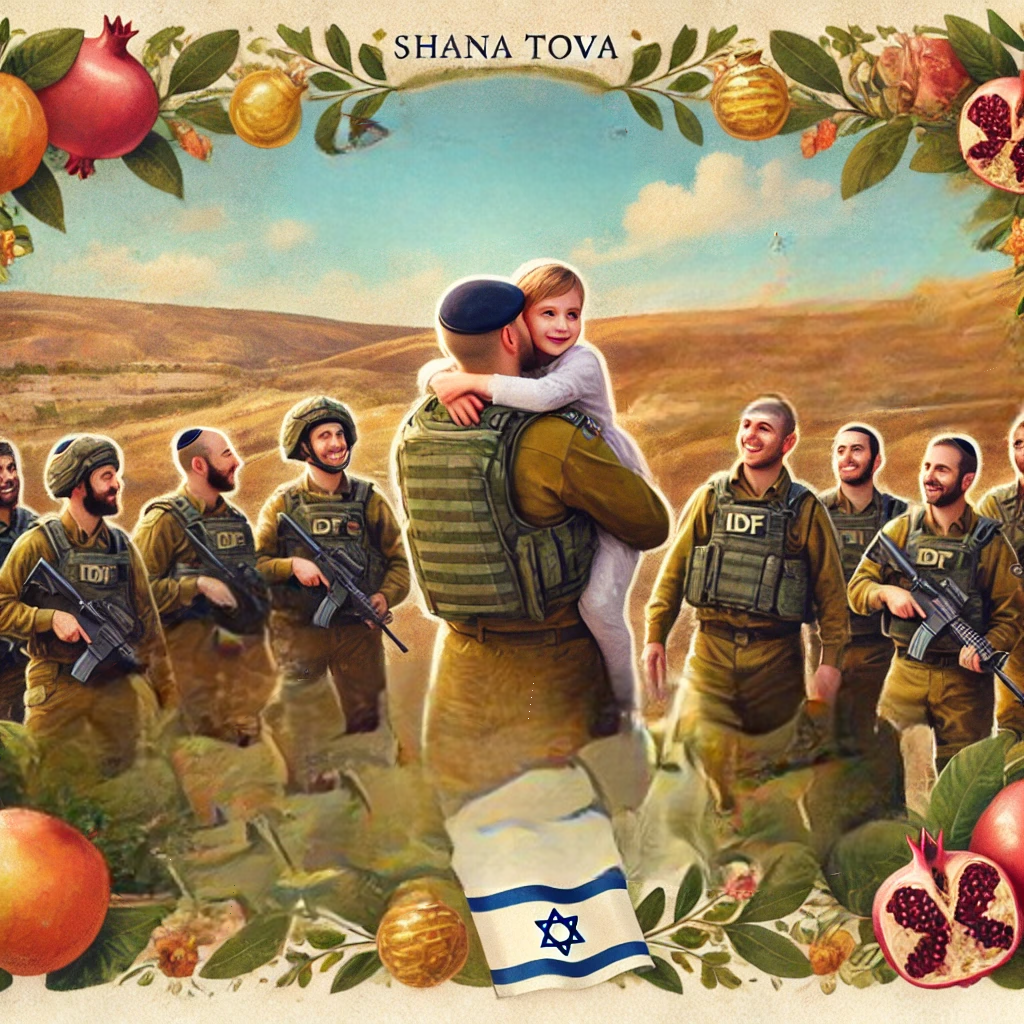
\includegraphics[scale=0.17]{his.png}
	\end{center}
\end{document}